\begin{figure}[!h]
  \centering
  \begin{adjustbox}{scale=0.8}
    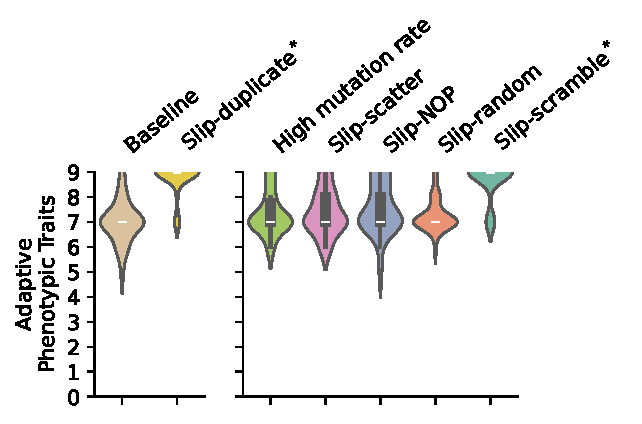
\includegraphics[
        height=4in,
        trim={0.2cm -1.5cm 0.2cm 0},
        clip
      ]{binder/binder/teeplots/col=split+env=static+hue=treatment+inner=box+kind=violin+palette=set2-r+viz=catplot+x=treatment+y=tasks-present+ext=.pdf}%
    \hspace*{-2.0cm}%
    \raisebox{0.125in}{%
      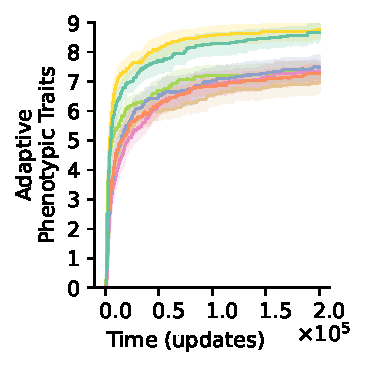
\includegraphics[
          height=2.7in,
          trim={1.36cm -0.64cm 0 0},
          clip
        ]{binder/binder/teeplots/env=static+errorbar=ci+exp=below+hue=treatment+kind=line+palette=set2-r+viz=relplot+x=time-100k+y=tasks-present+ext=.pdf}}%
  \end{adjustbox}

  \vspace{-7ex}

  \begin{subfigure}{0.3\textwidth}
    \caption{\small slip-duplication}
    \label{fig:results_panels:slip_duplication}
  \end{subfigure}%
  \begin{subfigure}{0.35\textwidth}
    \caption{\small ablation treatments}
    \label{fig:results_panels:ablation}
  \end{subfigure}%
  \begin{subfigure}{0.22\textwidth}
    \caption{\small lineage history}
    \label{fig:results_panels:time_series}
  \end{subfigure}

  \vspace{1ex}

  \caption{\textbf{Treatments preserving slip-duplicated content facilitate adaptive evolution.}
    \small Violin plots show number of adaptive traits evolved in final dominant genotypes.
    Time series (\ref{fig:results_panels:time_series} right) shows progression of adaptive phenotypic trait counts along lineages of final dominant genotypes; color-coding corresponds to violin plots.
    Asterisk (*) markers indicate treatments with significantly more adaptive phenotypic traits compared to baseline, comparison across both panels \ref{fig:results_panels:slip_duplication} and \ref{fig:results_panels:ablation}.
    Simulation time unit is “updates,” corresponding to evaluation of ~30 genome sites per organism.}
  \label{fig:results_panels}
\end{figure}
